\section{Quasielastic Scattering and the Glauber Approximation}
Benhar et. al~\cite{Benhar_2000, Rohe_2005} present a calculation of nuclear
transparency for quasielastic scattering in the correlated Glauber
approximation.
What follows is a summary of their method.

Let
$\Psi_0^{(A)}$ be the ground state wave function of the $A$-body target nucleus,
$\Psi_{\vec{p}}$ the final state wave function of the ejected proton with momentum $\vec{p}$,
and
$\Psi_f^{(A-1)}$ is the final state wave function of the residual $(A-1)$ nucleus.
Then, in terms of
annihilation $\hat{a}_{\vec{k}}$ and
creation operators $\hat{a}_{\vec{k}}^\dagger$
for nucleon states of momentum $\vec{k}$,
the matrix amplitude for $A(e,e'p)$ scattering can be
written
\begin{equation}
    \mathcal{M} = \braopket{\Psi_{\vec{p}}^{(A-1)}}
                           {\sum_{\vec{k}} \hat{a}^\dagger_{\vec{k}+\vec{q}} \hat{a}_{\vec{k}}}
                           {\Psi_0^{(A)}}
\end{equation}


The Hamiltonian of the full $A$-body system can be rewritten to separate the
final state interactions between the ejected proton and the spectator nucleons
\begin{equation}
    \hat{H}_{A} = \hat{H}_0 + \hat{H}_{FSI} = (\hat{H}_{A-1} + T_1) + \hat{H}_{FSI}
\end{equation}
where $H_{A_1}$ is the Hamiltonian of the recoil nucleus
$T_1$ is the kinetic energy operator for the ejected proton
and
$\hat{H}_{FSI}$ contains the final state interactions.


Then, if the state $\Phi_{\vec{p}}$ is an eigenstate of $H_0$ that describes
the system in the absence of FSI, there is a scattering operator
$\Omega_{\vec{p}}$ such that
\begin{equation}
    \ket{\Psi_{\vec{p}}} = \Omega_{\vec{p}} \ket{\Phi_{\vec{p}}}
\end{equation}


Formally, this operator can be written
\begin{align}
    \Omega_{\vec{p}} &= \lim_{t\rightarrow\infty} e^{-i\hat{H}_At}e^{-i\hat{H}_0t} \\
                     &= \lim_{t\rightarrow\infty} \hat{T} e^{-\int_0^t dt' \hat{H}_{FSI}(t')}
\end{align}
where $\hat{T}$ is the time ordering operator and
\begin{equation}
    \hat{H}_{FSI}(t) = e^{i\hat{H}_0t} \hat{H}_{FSI} e^{-i\hat{H}_0t}
\end{equation}

Calculating this expression for a realistic Hamiltonian is difficult, but under
appropriate circumstances the Glauber approximation~\cite{Glauber_1959} can be
used to simplify this expression.
The Glauber approximation assumes that
the ejected proton moves in a straight line without rescattering
(the eikonal approximation)
and
the spectator nucleons can be treated as fixed
(the frozen approximation).

Assume the spectator nucleons are frozen at positions
$\vec{r}_j = z_j \hat{z} + \vec{b}_j$
where the $\hat{z}$ axis lies along the path of the ejected proton
and $\vec{b}_j$ are perpendicular to $\hat{z}$.

Let $R=\left\{ \vec{r}_1,\vec{r}_2,\ldots,\vec{r}_A \right\}$ be the
spatial configuration of the full $A$-body system.
In the correlated Glauber approximation, the scattering operator can be written
in coordinate space
\begin{align}
    \Omega_{\vec{p}}(R) \equiv \braopket{R}{\Omega_{\vec{p}}}{R}
        = \hat{P}_z \bigg[ 1 &- \sum_{j=2} \theta(z_j-z_1) \Gamma(\vec{b}_j-\vec{b}) \nonumber \\
                        &+ \sum_{j=2,k>j} \theta(z_j-z_1) \Gamma(\vec{b}_j-\vec{b}) \theta(z_k-z_1) \Gamma(\vec{b}_k) \nonumber \\
                        &- \cdots \bigg]
\end{align}
where $\hat{P}_z$ is a $z$-ordering operator preventing backscattering of the
ejected proton and the step functions $\theta(z)$ ensure causality.
The profile function $\Gamma(\vec{b})$ is a function of impact parameter
$\vec{b}$ and contains all the information about the scattering process.
It is a Fourier transform of the scattering amplitude $f(\vec{k}_t)$ which can
be extracted from measured cross sections.
\begin{equation}
    \Gamma(\vec{b}) = -\frac{i}{2}\int \frac{d^2k_t}{(2\pi)^2} e^{-\vec{k}_t \cdot \vec{b}} f(\vec{k}_t)
\end{equation}

The scattering amplitude takes the parameterized form
\begin{equation}
    f(\vec{k}_t) = i \sigma_{tot} (1-i\epsilon) e^{-k_t^2/2B}
\end{equation}
where $\epsilon$ is the ratio of the scattering amplitude's real and imaginary
parts and
$B$ is a slope parameter.

Let $\rho_p(\vec{r})$ be the proton density in a target nucleus with $Z$
protons.
Then the transparency is
\begin{equation}
    T = \frac{1}{Z} \int d^3r \rho(\vec{r}) \left| \Omega_{\vec{p}}(\vec{r})\right|^2
\end{equation}

The integrand can be expanded in terms of $n$-body distribution functions
$\rho^{(n)}_{p N \ldots N}(\vec{r}_1, \vec{r}_2, \cdots, \vec{r}_n)$ that express the
joint probability of finding the ejected proton at $\vec{r}_1$ and the $n-1$
spectator nucleons at positions $\{\vec{r}_2, \cdots, \vec{r}_n\}$.

\begin{align}
    \rho_{p}(\vec{r}_1)&\left| \Omega_{\vec{p}}(\vec{r})\right|^2 = \nonumber \\
        &1 - \frac{1}{\rho_{p}(\vec{r}_1)} \bigg[ \int d^3 \vec{r}_2 \theta(z_2-z)\Gamma(\vec{b}_2-\vec{b}) \rho^{(2)}_{pN}(\vec{r}_1,\vec{r}_2) \nonumber \\
            - &\int d^3 \vec{r}_2 d^3 \vec{r}_3 \theta(z_2-z)\Gamma(\vec{b}_2-\vec{b}) \theta(z_3-z)\Gamma(\vec{b}_3-\vec{b}) \rho^{(3)}_{pNN}(\vec{r}_1,\vec{r}_2, \vec{r}_3) \nonumber \\
            + &\int d^3 \vec{r}_2 d^3 \vec{r}_3 d^3 \vec{r}_4 \cdots \bigg]
\end{align}

The quantity in brackets contains the effects of final state interactions,
which result in a decrease in transparency from the PWIA result, $T=1$.
Each term represents a contributions from $n-1$ rescatterings.
The single rescattering term can be written as
$\rho^{(2)}_{pN}(\vec{r}_1,\vec{r}_2)=\rho_p(\vec{r}_1)\rho_N(\vec{r}_2)g(\vec{r}_1,\vec{r}_2)$,
where the function $g(\vec{r}_1,\vec{r}_2)$ describes the correlations between
nucleons~\cite{Schiavilla_1987}.
At short ranges $r=\norm{\vec{r}_1-\vec{r}_2}$, $g(r)\ll1$ because of the
strongly repulsive core of the nucleon-nucleon interaction.
At large $r$, $g(r) \rightarrow 1$ because of asymptotic freedom.

\subsection{Pandharipande et al.}
%The Glauber approximation~\cite{Glauber_1959} supposes that a struck proton
%with momentum $k$ and energy $E$, after quasielastic scattering, subsequently
%scatters from spectator nucleons at angles $\theta$ primarily in the
%forward direction.
%More precisely, if $a$ and $V$ are the radius and strength of the
%nucleon-nucleon interaction, this requires
%$V/E \ll 1$,
%$ka \gg 1$,
%and
%$\theta^2 k a \ll 1$.
%The wavefunction of the proton in these conditions can be written as
%%TODO: clean this up a little and clarify some variables; I'm trying to draw a link between a general Glauber summary and the specifics of the Pandharipande/Pieper paper
%\begin{equation} \label{eqn:eikonal_approximation}
%    \psi(\vec{r}) = e^{i\vec{k}\cdot\vec{r}}
%            \exp{ -\frac{1}{2} \int_{z'}^{z} dz'' \sigma(z'') \rho(\vec{r''}) }
%\end{equation}


This experiment takes the work of Pandharipande and
Pieper~\cite{Pandharipande_1992} as the null hypothesis against which the onset
of color transparency is to be tested.
This is the same model used in previous measurements of nuclear transparency
in quasielastic
scattering~\cite{Garrow_2002,Abbot_1998,Rohe_2005,Garino_1992}.
%NB: Makins_1994 uses Benhar_1992, not Pandharipande_1992.
%NB: ONeill_1995 doesn't really use one explicitly?; they just reference qualitative features

% TODO: clean this up a lot. This is basically my notes on the paper.
The model starts with the assumption that the differences between cross
sections for free and in-medium nucleon-nucleon scattering arise primarily from
Pauli blocking of final states and effective mass corrections.
Pandharipande and Pieper find good agreement between experimental results and
their model's estimates of the imaginary part of the optical potential in
nuclear matter.
The model uses the
Urbana $\text{v}_{14}+\text{TNI}$ Hamiltonian~\cite{Lagaris_1981_331, Lagaris_1981_349}
and variational method~\cite{Wiringa_1988, Friedman_1981}
to calculate an optical potential $U$ for symmetric nuclear matter.
This Hamiltonian includes the effect of nucleon-nucleon correlations by fitting
two-body operators to phase shift data taken for neutron-proton
scattering~\cite{Arndt_1966}.


The dispersion relation $e(k,\rho)$ for nucleons in nuclear matter with density
$\rho$ and real part of the optical potential $U(k,\rho)$ is
\begin{equation}
    e(k,\rho) = \frac{\hbar^2 k^2}{2m} + U(k,\rho)
\end{equation}

% as opposed to phase velocity
The group velocity of an in-medium nucleon with momentum $k$ differs from that of a
free nucleon.
The derivative of the dispersion relation gives this velocity and a
definition of the effective mass $m^*$
\begin{equation}
    \frac{1}{\hbar}\frac{d}{dk}e(k,\rho)
        = \frac{\hbar^2 k}{m} + \frac{1}{\hbar}\frac{d}{dk}U(k,\rho)
        \equiv \frac{\hbar k}{m^*(k,\rho)}
\end{equation}

% With this velocity $v'$, transition matrix $t'$, and density of states $D'$,
% the in-medium nucleon-nucleon scattering cross section in a volume of size
% $L^3$ can be expressed as
% \begin{equation}
%     \frac{d\sigma}{d\Omega} = \frac{L^3}{v'} \frac{2\pi}{\hbar} |t'|^2 D'
% \end{equation}
% The equivalent expression holds with unprimed quantities for the vacuum cross
% section.
% Assuming the in-medium correlated two-nucleon wave function at small
% interparticle distances is the same as in the vacuum, the transition matrix
% $t'$ can be taken to be $t' \approx t$.
% Using the approximation from Ref~\cite{Krotscheck_1981}, the in-medium density
% of states is
% \begin{equation}
%     D' = D \frac{m^*\left( \sqrt{\frac{1}{2}(k_3^2+k_4^2)}, \rho \right)}{m}
% \end{equation}
% and the in-medium differential cross section is
% \begin{equation}
% \begin{aligned}
%     \frac{d \sigma^{\prime}}{d \Omega}=& \frac{v_{\mathrm{rel}}}{v_{\mathrm{rel}}^{\prime}} \frac{D_{f}^{\prime}}{D_{f}} \frac{d \sigma}{d \Omega} \\
%     =& \frac{\left|\mathbf{k}_{1}-\mathbf{k}_{2}\right|}{m}\left[\left|\frac{\mathbf{k}_{1}}{m^{*}\left(k_{1}, \rho\right)}-\frac{\mathbf{k}_{2}}{m^{*}\left(k_{2}, \rho\right)}\right|\right]^{-1} \\
%     & \times \frac{m^{*}\left[\sqrt{\left(k_{3}^{2}+k_{4}^{2}\right) / 2}, \rho\right]}{m} \frac{d \sigma}{d \Omega}
% \end{aligned}
% \end{equation}

The in-medium cross section for a proton with momentum $k$ scattering off a
nucleon $a=n,p$ is
\begin{equation}
    \widetilde{\sigma}_{pa}(k,\rho)=\frac{m^{*}(k, \rho)}{\hbar k \rho_{a} \tau_{a}(k)}
\end{equation}
where $\tau_a$ is the life time of the two-particle-one-hole state.
With this expression for the cross section, the nuclear transparency $T$ can be
calculated using a local density approximation and a wavefunction from
conventional Glauber multiple-scattering theory,
\begin{equation}
    T=\frac{1}{A} \int d^3r' \rho_{p}(\vec{r'}) P_{T}(\vec{r'})
\end{equation}
where $P_T$, the probability that a proton struck at $\vec{r'}$ emerges without
rescattering, is

% with align
\begin{equation}
\begin{aligned}
    P_{T}(\vec{r'}) = \exp \biggl\{-\int_{z'}^{\infty} dz'' \biggr.\biggl[&g_{p n}(\vec{r'}, \vec{r''}) \widetilde{\sigma}_{p n}\left(k, \rho(\vec{r''})\right) \rho_{n}(\vec{r''})\biggr.\\
                                                           \biggl.\biggl.+&g_{p p}(\vec{r'}, \vec{r''}) \widetilde{\sigma}_{p p}\left(k, \rho(\vec{r''})\right) \rho_{p}(\vec{r''})\biggr]\biggr\}
\end{aligned}
\end{equation}

% % one long line
% \begin{equation}
%     P_{T}(\vec{r'}) =
%     \exp \left\{
%         -\int_{z'}^{\infty} dz'' \left[
%             g_{pn}(\vec{r'},\vec{r''})\widetilde{\sigma}_{pn}(k, \rho(\vec{r''})) \rho_{n}(\vec{r''})
%             +
%             g_{pp}(\vec{r'},\vec{r''})\widetilde{\sigma}_{pp}(k, \rho(\vec{r''})) \rho_{p}(\vec{r''})
%         \right]
%     \right\}
% \end{equation}

In the above expression, $g_{pa}(\vec{r'},\vec{r''})$ is a pair distribution
function~\cite{Schiavilla_1987}, the joint probability to find a proton at
$\vec{r'}$ and nucleon $a$ at $\vec{r''}$.

Glauber models such as this predict that nuclear transparency $T$ remains
constant for increasing momentum transfer $Q^2$, as shown by the dotted line in
Fig~\ref{fig:aeep_transparency_intro}.

% TODO: Do we have a PDF version of this?
\begin{figure}[!h]
    \centering
    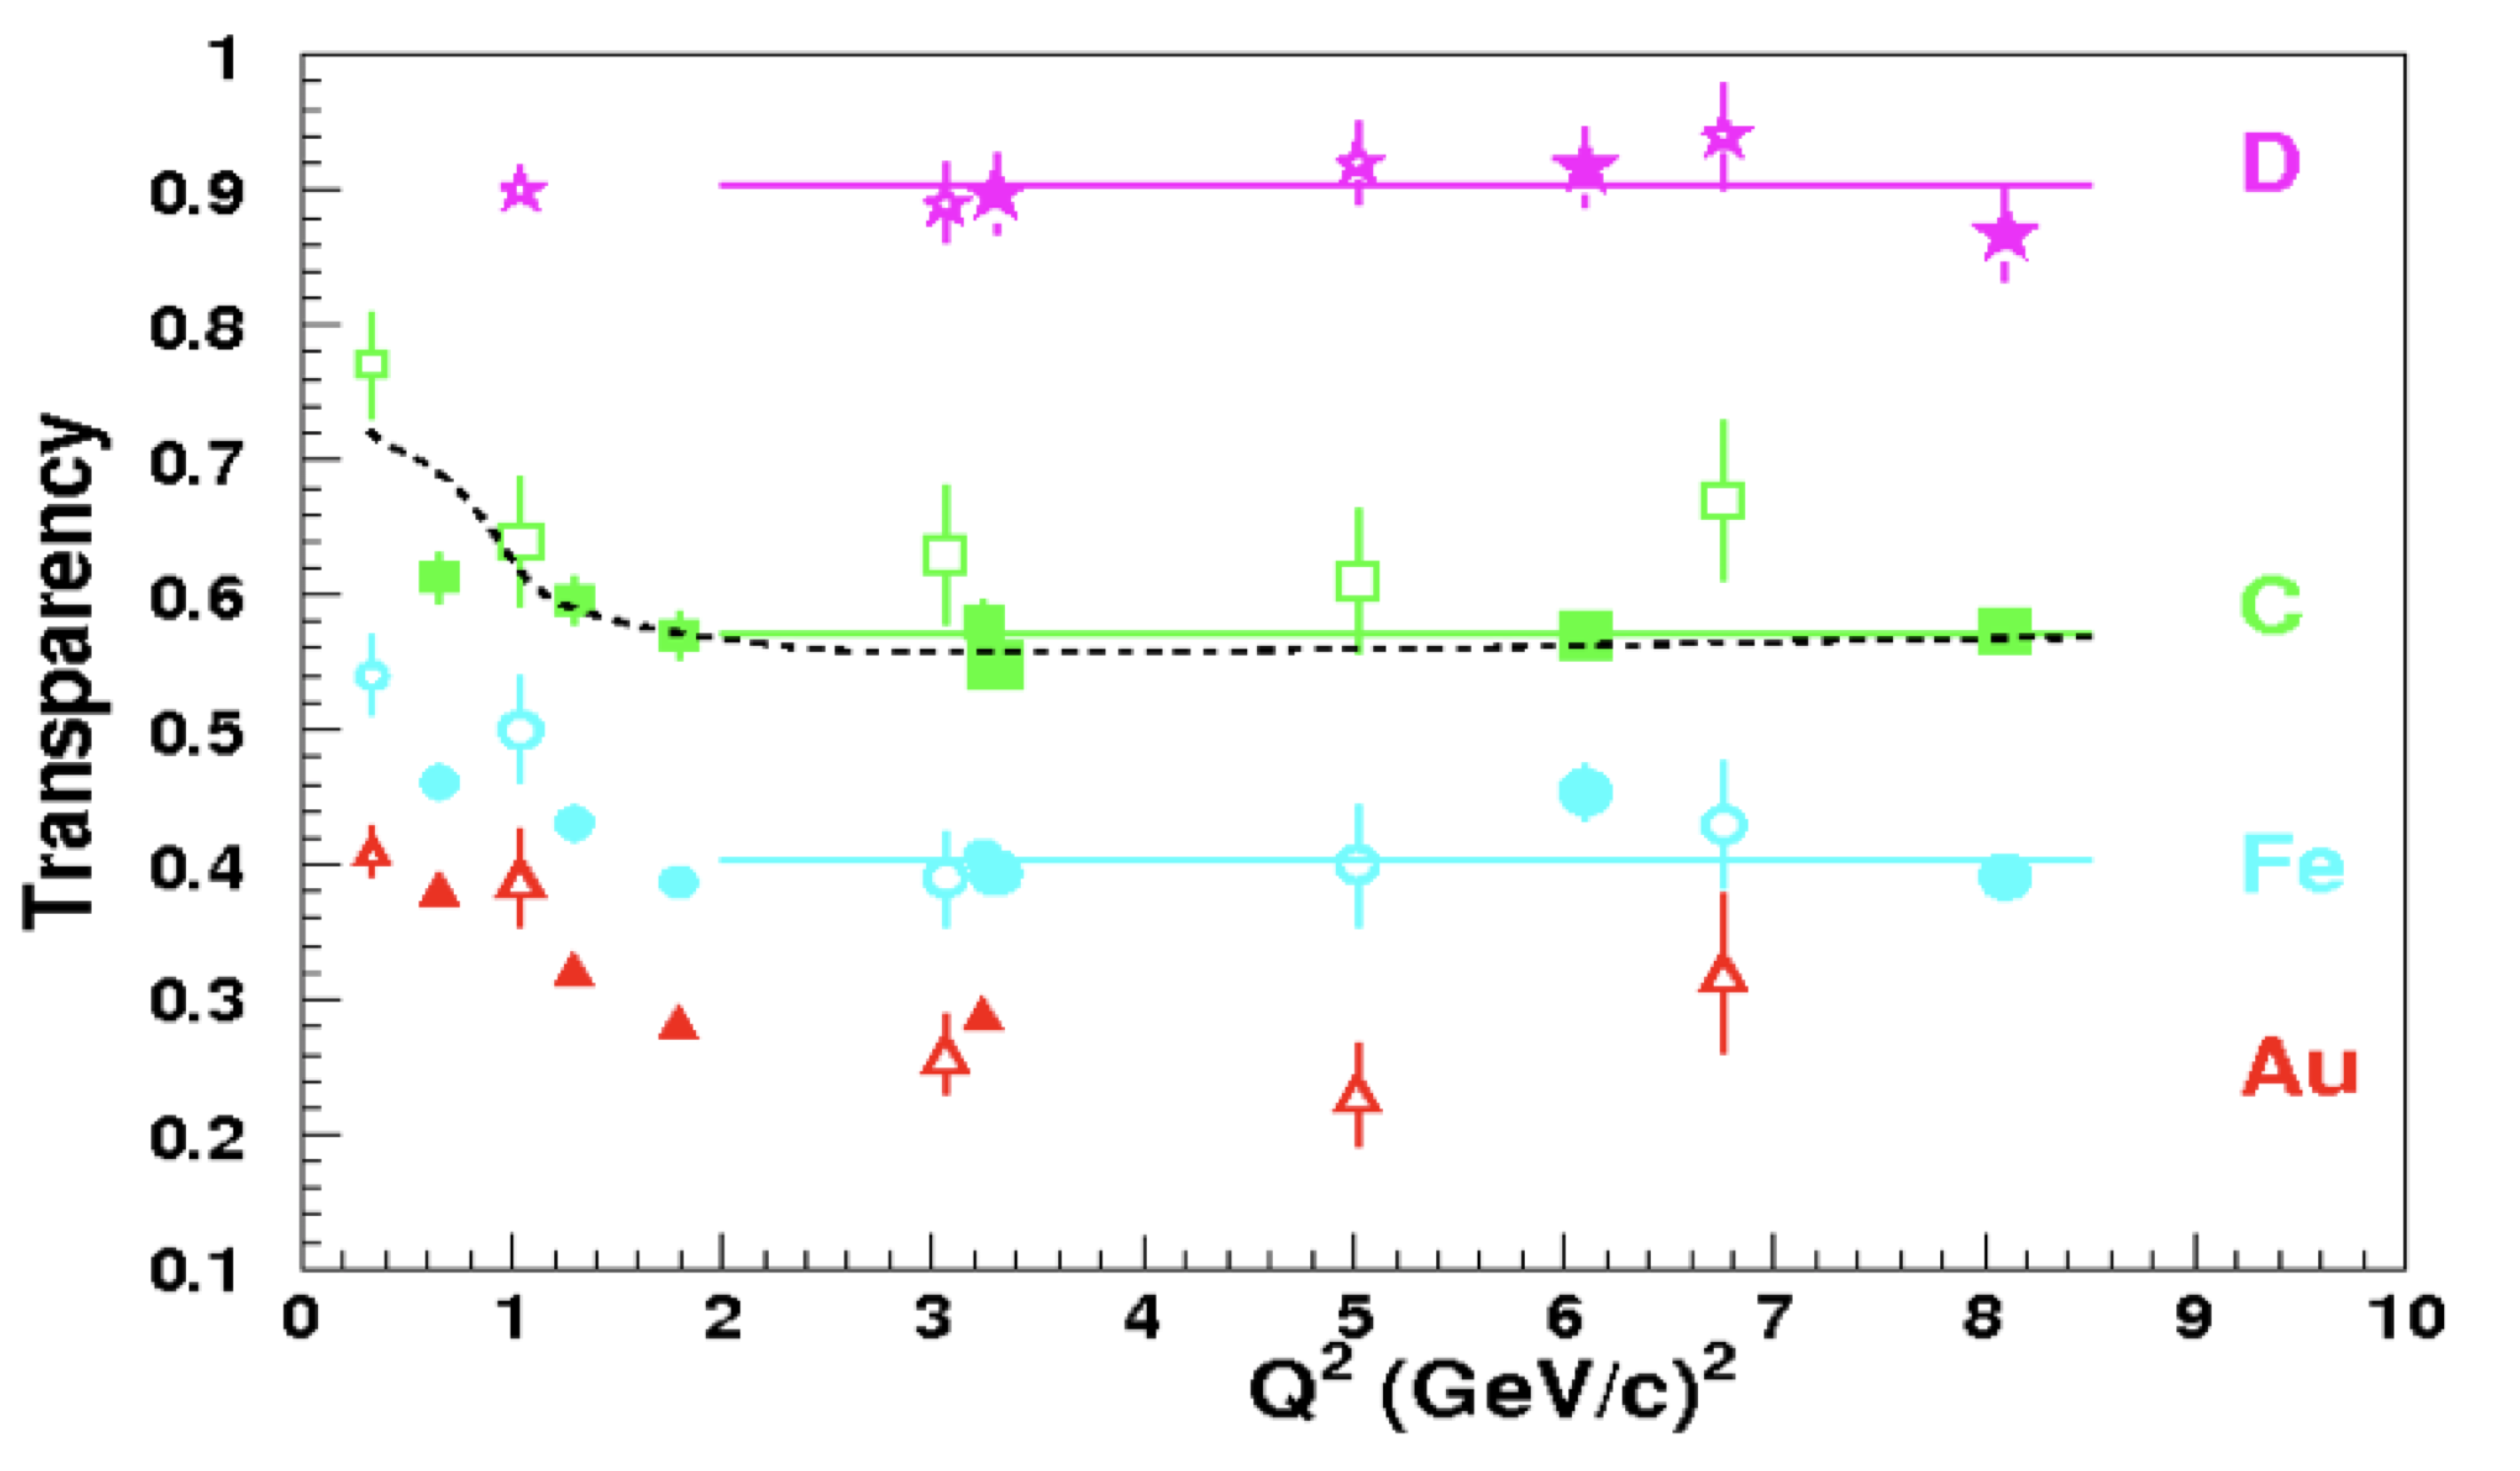
\includegraphics[width=0.6\textwidth]{chap2/aeep_transparency.png}
    \caption{Transparency measurements from several experiements studying
             quasielastic electron scattering from deuterium, carbon, iron,
             and gold.
             Data taken at JLab~\cite{Abbot_1998, Garrow_2002, Rohe_2005} are shown as solid points.
             Data taken at SLAC~\cite{Makins_1994, ONeill_1995} are shown as large open symbols.
             Data taken at Bates~\cite{Garino_1992} are shown as small open symbols.
             The dotted line is a Glauber calculation from~\cite{Pandharipande_1992} for carbon data.
             Solid lines are constant-value fits to data above \SI{2}{\giga\electronvolt}.
            }
    \label{fig:aeep_transparency_intro}
\end{figure}


